%
% File coling2014.tex
%
% Contact: jwagner@computing.dcu.ie
%%
%% Based on the style files for ACL-2014, which were, in turn,
%% Based on the style files for ACL-2013, which were, in turn,
%% Based on the style files for ACL-2012, which were, in turn,
%% based on the style files for ACL-2011, which were, in turn, 
%% based on the style files for ACL-2010, which were, in turn, 
%% based on the style files for ACL-IJCNLP-2009, which were, in turn,
%% based on the style files for EACL-2009 and IJCNLP-2008...

%% Based on the style files for EACL 2006 by 
%%e.agirre@ehu.es or Sergi.Balari@uab.es
%% and that of ACL 08 by Joakim Nivre and Noah Smith

\documentclass[11pt]{article}
\usepackage{coling2014}
\usepackage{times}
\usepackage{url}
\usepackage{latexsym}
\usepackage{graphicx}
\usepackage{caption}
\usepackage{subcaption}
\usepackage{multibib}

%\setlength\titlebox{5cm}

% You can expand the titlebox if you need extra space
% to show all the authors. Please do not make the titlebox
% smaller than 5cm (the original size); we will check this
% in the camera-ready version and ask you to change it back.


\title{An Analysis of Multiword Expressions in the Paraphrase Database}

\author{First Author \\
  Affiliation / Address line 1 \\
  Affiliation / Address line 2 \\
  Affiliation / Address line 3 \\
  {\tt email@domain} \\\And
  Second Author \\
  Affiliation / Address line 1 \\
  Affiliation / Address line 2 \\
  Affiliation / Address line 3 \\
  {\tt email@domain} \\}

\date{}

\begin{document}
\maketitle
\begin{abstract}
We investigate whether paraphrases might be a useful resource for understanding multiword expressions (MWEs).  In particular, we analyze the paraphrases in PPDB, the Paraphrase Database, where multiple words are re-written as a single word.  By automatically mapping from multiword expressions onto single words, NLP systems could potentially process the re-written text more easily than the original text containing MWEs. We use the MWE categorization system as described in \newcite{Sag2002}.  Although a small proportion of the many-to-one paraphrases in PPDB are classic MWEs, the resource contains millions of entries.  We therefore train a classifier to distinguish interesting MWEs from other sorts of many-to-one paraphrases.
\end{abstract}

\section{Introduction}
\label{intro}

%
% The following footnote without marker is needed for the camera-ready
% version of the paper.
% Comment out the instructions (first text) and uncomment the 8 lines
% under "final paper" for your variant of English.
% 
\blfootnote{
    %
    % for review submission
    %
    \hspace{-0.65cm}  % space normally used by the marker
    Place licence statement here for the camera-ready version, see
    Section~\ref{licence} of the instructions for preparing a
    manuscript.
    %
    % % final paper: en-uk version (to license, a licence)
    %
    % \hspace{-0.65cm}  % space normally used by the marker
    % This work is licensed under a Creative Commons 
    % Attribution 4.0 International Licence.
    % Page numbers and proceedings footer are added by
    % the organisers.
    % Licence details:
    % \url{http://creativecommons.org/licenses/by/4.0/}
    % 
    % % final paper: en-us version (to licence, a license)
    %
    % \hspace{-0.65cm}  % space normally used by the marker
    % This work is licenced under a Creative Commons 
    % Attribution 4.0 International License.
    % Page numbers and proceedings footer are added by
    % the organizers.
    % License details:
    % \url{http://creativecommons.org/licenses/by/4.0/}
}

Multiword expressions (MWEs) are phrases whose meanings are different than the literal interpretation of the words in the phrase. MWEs include verb-particle constructions, fixed expressions, compound nominals, and decomposable idioms, to name a few \cite{Sag2002}.  MWEs are difficult to process both for non-native speakers of English, as well as for NLP systems. Studies using an eye-movement paradigm have found that non-native speakers of English required more time to retrieve figurative senses of phrases than literal ones, whereas native speakers retrieved the idiomatic meaning faster than the literal meaning \cite{siyanova-chanturia-martinez:2014}. These studies imply that L2 speakers of English may find it more difficult to understand MWEs than a similar phrase whose meaning was literal.  Among NLP systems, both parsers and information retrieval systems make errors on MWEs. As described by \newcite{Villavicencio2007}, \newcite{Baldwin2004} found that, among a random sample of 20,000 strings from the written portion of the British National Corpus \cite{Burnard2000}, using the English Resource Grammar \cite{Copestake+Flickinger2000}, MWEs caused 8\% of all parse errors. When manually selected compound nominals were searched for as single terms it improved information retrieval results \cite{Acosta2011}.

Because MWEs are challenging for many NLP tasks, automatically identifying them could be useful for identifying and averting errors.  Several research efforts have examined this topic.  For example, \newcite{muzny-zettlemoyer:2013:EMNLP} built a classifier to identify idioms, and \newcite{li-sporleder:2010:NAACLHLT} use Gaussian Mixture Models to identify new idioms.  In this paper, we use the Paraphrase Database (PPDB) as a resource to define a MWE lexicon, which could be incorporated into other NLP systems.  In addition to being a potentially useful resource for {\it identifying} MWEs, it has the unique feature of potentially giving an {\it interpretation} of the MWEs by replacing them with a one word paraphrase.  

In this paper we
\begin{itemize}
\item Analyze the PPDB for the prevalence of various types of MWEs
\item Build a classifier that distinguishes interesting MWEs in the PPDB from more generic paraphrases
\item Investigate whether parse quality can be improved by substituting MWEs with one word paraphrases
\end{itemize}

\section{The Paraphrase Database}

The Paraphrase Database (PPDB) is a database containing English paraphrases. PPDB was developed using alignment techniques from machine translation on bilingual parallel corpora, pivoting on a foreign language, to find English phrases that translate to the same foreign-language phrase \newcite{bannard-callisonburch:2005:ACL}. The database takes into account syntactic information of both the English and foreign-language phrases: the entries in PPDB were found using SCFGs to come up with paraphrases that form constituents of the same syntactic category \cite{ganitkevitch-EtAl:2011:EMNLP,ganitkevitch-vandurme-callisonburch:2013:NAACL-HLT}.

\section{Related Work}

Various definitions of MWEs have been used for NLP tasks. Sag et al. define a taxonomy of multiword expressions that is widely used in computational MWE research. They define broad categories for MWEs (fixed expressions, semi-fixed expressions, syntactically flexible expressions, institutionalized phrases), and more specific categories within each of these. The following is a brief outline of the categories defined by Sag et al. that we investigate in this paper:

\begin{itemize}
\item Fixed expressions. These are expressions that don't fit standard grammar rules and are not compositional.

\item Non-decomposable idioms. These are expressions that follow grammatical rules, but whose meaning is not compositional.

\item Compoun nominal. Noun combinations whose meaning is different than the individual nouns in the phrase.

\item Proper nouns. These are included in the taxonomy because names allow for some kinds of variation but not others (e.g., the San Francisco 49ers, the 49ers, 49ers, but not the Oakland 49ers).

\item Decomposable idioms. 

\item Verb-particle constructions. These are verb phrases formed of a verb followed by a particle, where the meaning of the phrase is different than that of the verb alone.

\item Light verbs. These are verb phrases formed of a light verb (make, give, do), followed by a noun phrase.
\end{itemize}

Other work has described a division of MWEs extracted from paraphrases: one-to-many, many-to-one,  decomposable and non-decomposable \cite{dpm}. They also investigated using paraphrases to automatically extract multiword expressions. \cite{dpm} consider dependency-based paraphrases and parallel corpora-based paraphrases as sources for MWEs, finding that 34\% of the MWEs in the MSR manual word alignments of the RTE 2006 corpus were present in these resources (Brockett, 2007). 

\section{Experimental Design}
The Paraphrases Database (PPDB) contains English paraphrases. We have characterized a subset of the paraphrases found in the PPDB, according to categories of multi-word expressions (MWEs), syntactic changes in the expansion from a word to its paraphrase, and what parts of speech appear in the corpus. We also looked at how many of the paraphrases in the PPDB appear to be spurious.

The categories of MWEs we looked at were light verbs, verb-particle constructions, negation, and superlatives. We also included the categories for MWEs described in Sag et al: fixed expressions, non-decomposable idioms, compound nominals, proper names, and decomposable idioms. 

In addition to MWE categories, we also included categories for syntactic changes from a word to its paraphrase: change of tense followed by a paraphrase, nominalizations, infinitival to, adverbial modifier, one or more words the same as part of the original word, determiner followed by a one-word paraphrase, determiner followed by the plural form, and change of tense. Finally, we included acronyms, hypernym-hyponym pairs, times, extra punctuation marks, and numbers as categories, as well as unspecified expansions and bad paraphrases. 

\section{Results}

Of a random sample of 500 paraphrases from the L one-to-many paraphrase file, the most common types of paraphrase were expansions using the same morphological form (117 instances, or 23.4\%), determiner followed by a one-word paraphrase (86 instances, or 17.2\%), and paraphrases that did not fall into a particular category (62 instances, or 12.4\%). Of the sample, 43 were bad paraphrases (8.6\%). The full list of categories and the number of instances in each are in the table below.  

Of the 500 paraphrases in the random sample, 37 (7.4\%) fell into the MWE categories defined by Baldwin et al. Of these MWE paraphrases, the most common were verb-particle constructions (14 instances, or 37.8\%) , followed by proper names (7, or 18.9\%). There were no instances of compound nominals in the sample.

The full list of categories with the number of instances of paraphrases in each, as well as illustrative examples for each, are in the table below (Table 1). MWEs, as defined by \newcite{Sag2002}, are marked in bold. 

\begin{table}[h]
\begin{center}
\begin{tabular}{|l|r|l|}
\hline \bf Paraphrase Category & \bf Number of & \bf Examples \\ 
 & \bf instances & \\
 & \bf in sample & \\ \hline
determiner + one-word paraphrase & 86 & photographs, the images; duties, the responsibilities \\
expansion & 62 & suffocate, need air; cumbersome, time consuming \\
expansion, same morphological form & 47 & fun, sounds like fun; signs, signs and signals \\
change of tense + paraphrase & 43 & initiated, has undertaken; say, going to tell \\
inaccurate/bad paraphrase & 43 & iron, a par; also, do i\\
implicit/most common modifier & 41 & baghdad, iraqi capital baghdad; \\
&& enrichment, uranium enrichment \\
implicit type & 29 & training, training course; customs, customs offices \\
adverbial modifier& 27 & interesting, very interesting; more, even more \\
acronym & 21 & gpa, the global programme of action; cras, \\
&& credit-rating agencies \\
one or more words  & 17 &  anytime, any point; enslavement, slave labour \\
the same as part of original word & &\\
\bf verb-particle & 14  & torched, burnt down; done, carried out\\
determiner + plural & 9 & gloves, the glove; militaries, the military\\
\bf proper noun & 7 & markov, mr markov; karadzic, radovan karadzic\\
change of tense & 7 & changing, be changed; attain, be attained\\
\bf fixed expression & 6 & applied, put into effect; plenty, a whole host \\
superlative & 5 & notably, most particularly; best-known, most famous\\
copula & 5 & qualify, are eligible; reason, been right \\
\bf decomposable idiom & 4 & nuts, out of your mind; sleeping, get a good night's sleep\\
\bf light verb & 4  &  issued, made available; place, make way \\
number & 4 & 20, twenty of; 5,000, 5 000\\
infinitival to & 3 & track, to follow; answer, to reply \\
nominalization & 3 &  operation, proper functioning \\
negation & 2 & unused, not utilized; non-parties, not parties  \\
time variation & 2 & 7:00, seven hours; 2003/04, the 2003-04 fiscal year\\
punctuation & 2 & debt-servicing, debt servicing; what, somethin '\\
\bf non-decomposable idiom & 2 & furious, as mad as hell; entails, brings with it\\
alternate spelling & 1 & al-najaf, al nagaf\\
\bf compound nominal & 0 &\\
\hline
\end{tabular}
\end{center}
\caption{\label{font-table} Number of instances from each category in random sample of 500. }
\end{table}

The distribution of the syntactic categories from this random sample is depicted in Table \ref{sc-dist}. 

\begin{table}[h]
\begin{center}
\begin{tabular}{|l|l|l|}
\hline \bf Syntactic category & \bf Frequency in sample & \bf Frequency in PPDB-L \\ \hline
NP & 254 & 101563 \\
VP & 109 & 39380 \\
X & 39 & 17005 \\
ADJP & 27 & 14513 \\
ADVP & 16 & 5451 \\
S & 9 & 4103 \\
INTJ & 3 & 1730 \\
TOP & 4 & 1476 \\
NX & 2 & 1113 \\
PP & 1 & 532 \\
FRAG & 3 & 388  \\ 
SQ & 0 & 305 \\
SBAR & 0 & 165 \\
WHNP & 0 & 163 \\
WHADVP & 0 & 66 \\
QP & 0 & 39 \\
LST & 0 & 3 \\ 
SBARQ & 0 & 3 \\
CONJP & 0 & 1 \\
PRT & 0 & 1 \\
\hline
\end{tabular}
\end{center}
\caption{\label{sc-dist} Distribution of syntactic categories in random sample of 500 words from PPDB L, and in the entire PPDB L file, sorted by frequency in PPDB L. }
\end{table}

In both samples, the most common part of speech is NP, followed by VP. 

In addition to categorizing a random sample of paraphrases, we searched for instances of light verbs, verb-particle constructions, negation, comparatives, and superlatives. The light verbs were those with the verb “have”, “take”, “make”, “hold” or “give, ” followed by a noun phrase. The verb-particle constructions were any verbs followed by the particles “down”, “up”, “on”, “out”, “over” or “upon.” Negation instances had the word “not” either in the original or the expanded paraphrase. Comparatives had the word “more,” and superlatives had the word “most.”

To find instances of verb-particle constructions, we used the Linux command 'grep' and the regular expression ' particle\b' to find phrases where the potential particle was not the first word, and to ensure that it was not a substring of another word (e.g., 'onto' instead of 'on'). For example, to find potential instances of verb-particle constructions with the particle 'up', we ran the following command:
grep ' up\b' ppdb-1.0-l-o2m

We then determined manually whether the phrases found were verb-particle constructions. The potential particle was sometimes a preposition or adverb, in which case it did not fit into this MWE category. 

We used similar commands to find instances of the other paraphrase categories. A list of the commands used is in the following table:

\begin{table}[h]
\begin{center}
\begin{tabular}{|l|rl|}
\hline \bf Paraphrase category & \bf Search command & \\ \hline
verb-particle construction & grep ' up \textbackslash b' ppdb\textunderscore filename &\\
light verbs & grep '\textbackslash b make ' ppdb\textunderscore filename &\\
negation & grep '\textbackslash b not ' ppdb\textunderscore filename &\\
comparatives & grep '\textbackslash b more ' ppdb\textunderscore filename &\\
superlatives & grep '\textbackslash b most ' ppdb\textunderscore filename &\\
\hline
\end{tabular}
\end{center}
\caption{\label{font-table} Linux commands to search for paraphrases of different types. }
\end{table}

The results from these searches are summarized in the tables below. We considered only light verb phrases with no extra terms (e.g., 'have a word', but not 'have a word with you' or 'can i have a word').

\begin{table}[h]
\begin{center}
\begin{tabular}{|l|l|l|l|}
\hline \bf Light verb & \bf Number of light & \bf Number of light & \bf Matching verbs\\ 
 & \bf verb phrases & \bf verb phrases & \\ 
 & \bf  found by grep & & \\ \hline
make & 46 & 35 & make a call, make a decision, make a suggestion\\
have & 105 & 45 & have a ball, have a conversation, have a word\\
give & 11 & 4 & give a damn, give a reply\\
take & 48 & 33 & take a break, take a look, take a walk\\
hold & 3 & 1 & hold a debate\\
\hline
\end{tabular}
\end{center}
\caption{\label{font-table} Light verbs: number of potential light verb phrases found by grep, the number of these that turned out to be light-verb phrases, and some examples. }
\end{table}

\begin{table}[h]
\begin{center}
\begin{tabular}{|l|r|l|}
\hline \bf Particle & \bf Number of verb-particle  & \bf Number of verb-particle\\ 
 & \bf constructions found & \bf  phrases found by grep \\ \hline
up & 439 & 439 \\
about & 10 & 115 \\
around & 44 & 47 \\
back & 145 & 156 \\
down & 190 & 195 \\
in & 32 & 207 \\
off & 134 & 134 \\
on & 109 & 196 \\
out & 383 & 383 \\
over & 65 & 67 \\
\hline
\end{tabular}
\end{center}
\caption{\label{font-table} Verb-particle constructions. }
\end{table}

After manually identifying categories, we developed a classifier to automatically find paraphrases that are interesting to MWE researchers. We built the classifier to find the following categories of MWE: verb-particle construction; expansion, same morphological form; implicit/most common modifier; implicit type; light verb; fixed expression; non-decomposable idiom; proper noun; decomposable idiom; light verb. 

The features we used were whether a preposition appeared in the expansion of the paraphrase (feature value either 1 or 0), whether the original word appeared in the expansion, whether a light verb appeared in the expansion, and all of the scores from the PPDB (every number that appeared in the entry following an equal sign).

The prepositions and light verbs used for the features are listed in the table below.

\begin{table}[h]
\begin{center}
\begin{tabular}{|l|rl|}
\hline \bf prepositions &  'about', 'around', 'back', 'down', 'in', 'off', 'on', 'out', 'over', 'up'  &\\ \hline
\bf light verbs &  'give', 'have', 'hold', 'make', 'take' &\\
\hline
\end{tabular}
\end{center}
\caption{\label{font-table} Words used as features for classifier. }
\end{table}

We used an SVM classifier (libsvm) with these features on our sample of 500 words. With ten-fold cross-validation, the accuracy of the classifier was 75.4\%. By comparison, a baseline classifier that returns the majority class has an accuracy of 69.2\%. 

To determine whether a lexicon of paraphrases extracted from the PPDB would be useful for the task of parsing, we took a sample of 33 paraphrases that fall into the categories described by \newcite{Sag2002} (verb particle, fixed expression, non-decomposable idiom, compound nominal, proper name, decomposable idiom, and light verb) from the random sample of 500 words. We then did a Google search to find a sentence containing the expansion, selecting sentences where the part of speech matched that of the paraphrase, by manual inspection. We restricted the sentences to those less than 50 words long. We then created an equivalent sentence by replacing the expansion with the one-word paraphrase. We used the online demo of the Berkeley parser \cite{petrov-EtAl:2006:COLACL} to parse these sentence pairs, and manually evaluated the resulting parse trees for each sentence of the pair.

Of the 33 paraphrases sampled, 30 were correctly parsed using the one-word paraphrase, and 29 were correctly parsed using the expansion. 2 were parsed correctly for the one-word paraphrase but not for the expansion, 1 was parsed correctly for the expansion but not the one-word paraphrase, and 1 was parsed incorrectly for both. Figure \ref{avail} shows the trees for a case where the sentence containing the one-word paraphrase ("leverage") is parsed correctly, but the sentence containing the expansion ("avail myself of") is not. Figure \ref{avail} shows the trees for a case where the sentence containing the expansion ("leverage") is parsed correctly, but the sentence containing the one-word paraphrase ("avail myself of") is not. Figure \ref{issued} shows the trees for a case where the sentence containing the one-word paraphrase ("issued") is parsed correctly, but the sentence containing the expansion ("made available") is not. Figure \ref{place} shows the trees for a case where both sentences are parsed incorrectly.

\begin{figure}
\centering
\begin{subfigure}{.5\textwidth}
  \centering
  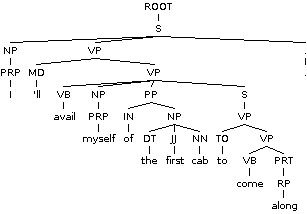
\includegraphics[width=80mm]{figs/avail_myself_of_tree.png}
  \caption{Original sentence: I'll avail myself of the first cab \\ to come along.}
  \label{fig:sub1}
\end{subfigure}%
\begin{subfigure}{.5\textwidth}
  \centering
  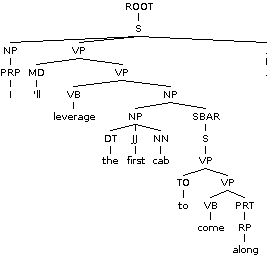
\includegraphics[width=58mm]{figs/leverage_tree.png}
  \caption{Sentence with substitution: I'll leverage the first cab to come along.}
  \label{fig:sub2}
\end{subfigure}
\caption{Parse trees for a sentence pair where substituting the single-word paraphrase for the MWE (in figure (b)) yields a better parse than the original sentence (in figure (a)).}
\label{avail}
\end{figure}


\begin{figure}
\centering
\begin{subfigure}{.5\textwidth}
  \centering
  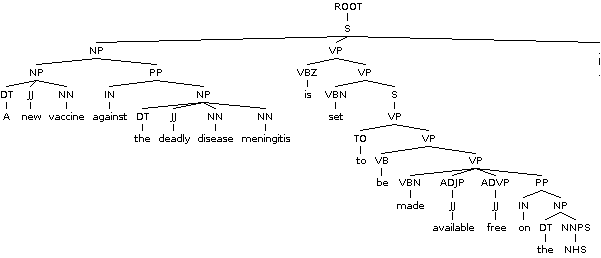
\includegraphics[width=80mm]{figs/made_available_tree.png}
  \caption{Original sentence: A new vaccine against the deadly \\
disease meningitis is set to be made available free \\
on the NHS.}
  \label{fig:sub1}
\end{subfigure}%
\begin{subfigure}{.5\textwidth}
  \centering
  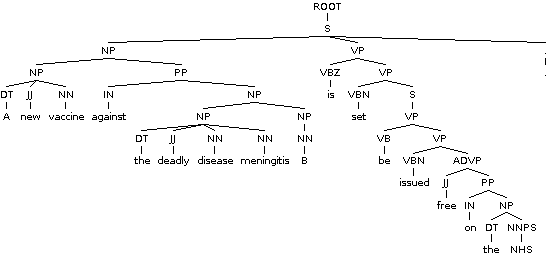
\includegraphics[width=73mm]{figs/issued_tree.png}
  \caption{Sentence with substitution: A new vaccine against the deadly disease meningitis is set to be issued free on the NHS.}
  \label{fig:sub2}
\end{subfigure}
\caption{Parse trees for a sentence pair where the original sentence (in figure (a)) yields a better parse than substituting the single-word paraphrase for the MWE (in figure (b)).}
\label{issued}
\end{figure}


\begin{figure}
\centering
\begin{subfigure}{.5\textwidth}
  \centering
  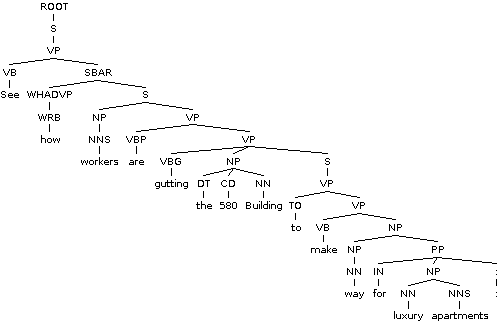
\includegraphics[width=80mm]{figs/make_way_tree.png}
  \caption{Original sentence:See how workers are gutting the \\
 580 Building to make way for luxury apartments.}
  \label{fig:sub1}
\end{subfigure}%
\begin{subfigure}{.5\textwidth}
  \centering
  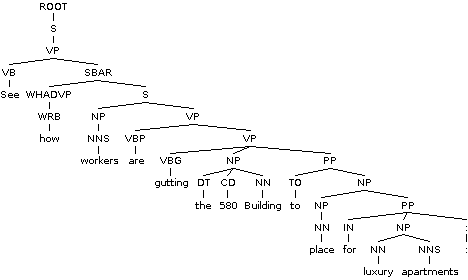
\includegraphics[width=87mm]{figs/place_tree.png}
  \caption{Sentence with substitution: See how workers are gutting the 580 Building to place for luxury apartments.}
  \label{fig:sub2}
\end{subfigure}
\caption{Parse trees for a sentence pair where the original sentence (in figure (a)) yields a better parse than substituting the single-word paraphrase for the MWE (in figure (a)).}
\label{place}
\end{figure}

%
% We are not doing the following for Coling 2014. Maybe next time.
%
% \section{XML conversion and supported \LaTeX\ packages}
% 
% ACL 2014 innovates over earlier years in that we will attempt to
% automatically convert your \LaTeX\ source files to machine-readable
% XML with semantic markup. This will facilitate future research that
% uses the ACL proceedings themselves as a corpus.
% 
% We encourage you to submit a ZIP file of your \LaTeX\ sources along
% with the camera-ready version of your paper. We will then convert them
% to XML automatically, using the LaTeXML tool
% (\url{http://dlmf.nist.gov/LaTeXML}). LaTeXML has \emph{bindings} for
% a number of \LaTeX\ packages, including the ACL 2014 stylefile. These
% bindings allow LaTeXML to render the commands from these packages
% correctly in XML. For best results, we encourage you to use the
% packages that are officially supported by LaTeXML, listed at
% \url{http://dlmf.nist.gov/LaTeXML/manual/included.bindings}

%\section*{Acknowledgements} 
%This material is based on research sponsored by the NSF under grant IIS-1249516 and DARPA under agreement number FA8750-13-2-0017 (the DEFT program). The U.S. Government is authorized to reproduce and distribute reprints for Governmental purposes. The views and conclusions contained in this publication are those of the authors and should not be interpreted as representing official policies or endorsements of DARPA or the U.S. Government.

% include your own bib file like this:
\section*{Bibliography}
\bibliographystyle{acl}
\bibliography{acl2014}


\end{document}
